\section{Reproducible verification and performance evidence}
\label{sec:experiments}

\subsection{What was measured and what was held fixed}

The experiments use the pinned repository source and the six additive modules
in this archive. Recorded hashes identify the actual implementation. The
runtime was CPython 3.12.14 on Linux x86-64. Regina's Python package version
was 7.4.1; its engine version string was 7.4. Plot generation used Matplotlib
3.10.8. Timing runs were serial, with no concurrent experiment launched by
this work. The shared host was not CPU-pinned, and the measurements are not
claims about a dedicated reference machine.

The normal-surface benchmark uses seven paired rounds after one warm-up call
per arm, with a fixed random seed and a randomized arm order in every round.
Every timed call validates its source, builds the relevant certificate, and
independently verifies it. Fixture construction, process startup, parsing the
saved input and final JSON serialization are outside the timed interval.
The full-coordinate arm also computes and certifies richer output than the
three-weight arm, while both answer the same disc-count question. The
reduced-count arm answers that question without claiming a full census of
the original vector. These output differences are intentional specializations
and should remain visible when comparing the timings.

The tables report median total times. A speed ratio is the median of the
seven within-round ratios, not the quotient of the two marginal medians.
An identical A/A arm measures ordinary run-to-run variation. No fitted
polynomial exponent or asymptotic complexity conclusion is inferred from
these finitely many times.

\subsection{Independent finite and large-binary oracles}

The abstract weighted-kernel audit checks 10,000 seeded finite interval
systems against literal union-find orbit sums and against the independent
checker. They comprise 299,040 literal points and 282,293 reduction events,
including 24,484 translation and 14,172 reflection pushes. Signed overlapping
weights, reversals, transmissions, both merger rules, and disconnected
supports are exercised. Eight closed-form systems extend the check through
20,000-bit universe sizes without expanding their points. The largest live
run list in this finite audit has 18 runs; this observation is evidence about
these fixtures, not a substitute for \cref{lem:weighted-run-growth}.

A separately written checker audit uses another deterministic seed and
2,500 literal union-find cases, 366 deliberate certificate mutations, and
81,412 reduction events. It includes a 20,002-bit endpoint case and two
producer-disabled replays. All pass. The delivered 103-method regression
selection includes the 30 new methods and 73 maintained interval and normal
backend methods; all pass from the portable bundle. This is the stated
selection, not a claim that the repository's entire application suite was
rerun.

The external audit uses Regina \cite{Regina} to construct and expand actual
normal surfaces. Expected component vectors, Euler characteristics,
orientabilities, boundary circles, boundary edge weights and disc predicates
come from that external implementation. The saved corpus contains raw face
pairings and expected component data, so it can be inspected without relying
on a verbal description of the fixtures.

\begin{center}
\begin{tabular}{lr}
\toprule
External normal-surface audit & Count \\
\midrule
Input normal vectors & 1,275 \\
Triangulations, including deterministic relabelings & 45 \\
Census comparisons across three query modes & 3,825 \\
Census-certificate replays & 3,825 \\
Canonical disc-count comparisons & 1,275 \\
Canonical disc-count certificate replays & 1,275 \\
Failed comparisons or replays & 0 \\
\bottomrule
\end{tabular}
\end{center}

The corpus includes 976 disconnected inputs, 252 with nonorientable
components, 778 with nontrivial quadrilateral gcd, and 537 with positive
vertex-link subtraction. There are 152 triangle-only inputs. It combines
layered solid tori, boundary caps with additional vertices, interior vertex
links, compatible mixtures of discs, spheres and M\"obius bands, finite
trefoil and figure-eight exteriors, and relabelings. The largest explicitly
expanded surface has 1,004 normal polygons and the largest triangulation has
10 tetrahedra; the configured expansion cap is 4,096 polygons. The large
binary tests and the external expanded audit therefore serve complementary
purposes.

\subsection{Two recorded counterexamples to aggregate tests}

The small separate counterexample file isolates cases that can be read and
replayed without opening the full corpus. In the one-tetrahedron solid-torus
case \code{lst_1_2:8}, the vector
\[
                    (2,2,0,0\,;\,0,0,2)
\]
is a union of two essential discs. Their total mod-two boundary class is
zero, while the componentwise count is two. The complete audit contains
198 inputs with essential discs but this total-homology cancellation.

In \code{interior_finite_trefoil:98}, an eight-tetrahedron finite trefoil
exterior contains the disjoint normal union of a four-polygon vertex-link
sphere and a 33-polygon once-punctured torus. The union is orientable, has
total Euler characteristic $2-1=1$ and nonzero total boundary class, and
contains no disc. Six orientable examples in the corpus have this latter
combination; ten do so without the orientability restriction. There are
72 inputs with positive total Euler characteristic but no disc component.
These cases demonstrate a correctness requirement that faster aggregate
arithmetic alone cannot meet.

\subsection{Actual normal-surface dimension comparison}

For $t\in\{4,8,16,32,64,128\}$, the benchmark supplies a primitive meridian
disc in a layered solid torus. The maintained fixture has
$F_{t+5}-5$ polygons, where $F_1=F_2=1$. At $t=128$ this is exactly
\[
        2\,791\,715\,456\,571\,051\,233\,611\,642\,548
\]
normal polygons. Its largest coordinate has only 89 bits. Both arms operate
on that compressed source, without building its expanded cell complex.

\begin{table}[htbp]
\centering\small
\setlength{\tabcolsep}{4pt}
\begin{tabular}{rrrrrr}
\toprule
$t$ & Input bits & Three weights (ms) & $7t$ weights (ms) & Paired ratio & A/A \\
\midrule
4 & 3 & 2.97 & 4.39 & 1.47 & 1.002 \\
8 & 6 & 6.37 & 13.69 & 2.17 & 1.003 \\
16 & 11 & 11.66 & 39.23 & 3.26 & 1.006 \\
32 & 22 & 58.55 & 268.36 & 4.71 & 1.090 \\
64 & 44 & 203.93 & 1728.48 & 9.21 & 0.992 \\
128 & 89 & 1152.80 & 12796.75 & 11.13 & 1.004 \\
\bottomrule
\end{tabular}

\caption{Actual normal-vector disc queries. Total milliseconds include
source validation, certificate production and independent replay. The ratio
compares full-coordinate extraction with the three-weight query; A/A compares
two identical three-weight arms.}
\label{tab:dimension}
\end{table}

The paired advantage increases from $1.47$ at four tetrahedra to $11.13$ at
128. At the last size, the median times are approximately 12.80 seconds and
1.15 seconds. Both use 133 orbit cycles: the improvement comes from weighted
work and result interpretation, not fewer discovery cycles. The observed
maximum run lists are 385 for full coordinates and eight for the three
statistics. Thus this particular family benefits both from smaller vector
dimension and a smaller weight-run representation. The theorem claims the
dimension reduction in the relevant arithmetic terms; it does not predict
that these wall-clock ratios must equal $7t/3$.

The normal benchmark's A/A paired ratios range from 0.990 to 1.090 across
both experiment families. The 32-tetrahedron run exhibits appreciable
variation. All samples are retained, and the graph shows their ranges. The
large-case improvements comfortably exceed the observed typical A/A
variation, but this small experiment is not a distributional study of knot
instances or a universal performance guarantee.

\subsection{Remove large coordinates even when the original gcd is one}

Fix the 16-tetrahedron meridian vector $D$ and boundary vertex link $L$, and
set
\[
 x_b=2^bD+(2^b+1)L,
 \qquad b\in\{64,512,4096,32768\}.
\]
The gcd of the original normal coordinates is one. Each input contains
exactly $2^b$ essential discs; the additional vertex-link discs have
inessential boundary. The core is always $D$, whose largest coordinate has
11 bits. The reduced route uses 21 orbit cycles at every size, compared with
39 for the direct three-weight query.

\begin{table}[htbp]
\centering\small
\setlength{\tabcolsep}{4pt}
\begin{tabular}{rrrrrr}
\toprule
$b$ & Input bits & Direct (ms) & Core (ms) & Paired ratio & A/A \\
\midrule
64 & 75 & 25.72 & 13.60 & 1.87 & 0.997 \\
512 & 523 & 27.80 & 13.87 & 2.00 & 1.011 \\
4,096 & 4,107 & 43.80 & 14.59 & 3.02 & 0.999 \\
32,768 & 32,779 & 169.70 & 21.81 & 7.64 & 0.990 \\
\bottomrule
\end{tabular}

\caption{Canonical reduction for $x_b=2^bD+(2^b+1)L$. Both routes count the
original input's essential discs and independently verify their evidence.
The core always has 11-bit coordinates. A/A compares identical core arms.}
\label{tab:core}
\end{table}

At $b=32768$, the largest input coordinate has 32,779 bits. The median total
times are 169.70 ms directly and 21.81 ms through the core, with a paired
median ratio of 7.64. Serialized proof sizes are approximately 4,417 KiB and
55 KiB, respectively. The outer core certificate still records large input
multiplicities, so it grows with $b$ even though the internal core orbit
proof is fixed. Likewise the reduced total runtime is not constant: reading,
validating, subtracting, taking the gcd, dividing and binding the original
source remain necessary.

\begin{figure}[htbp]
\centering
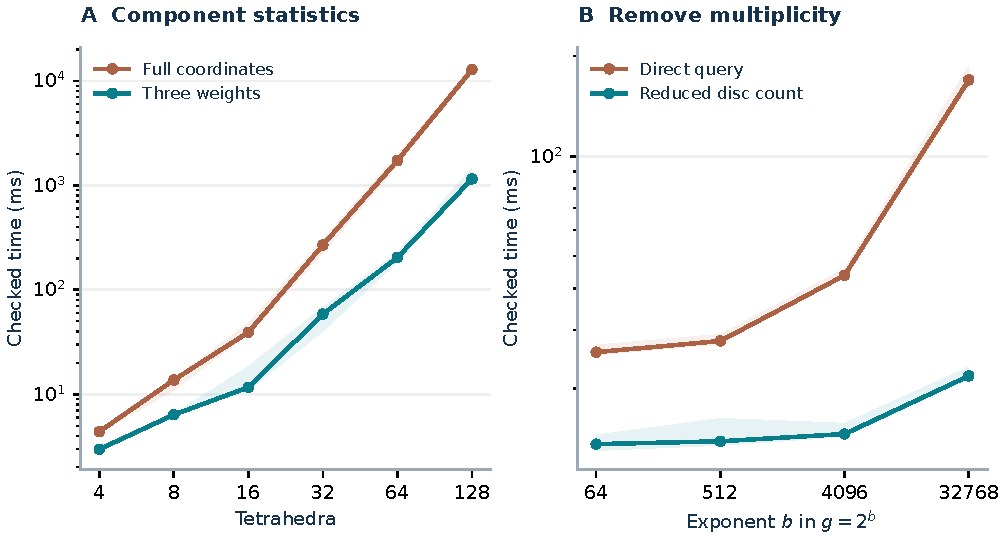
\includegraphics[width=\linewidth]{figures/normal_query_benchmarks.pdf}
\caption{Checked query times from the archived raw samples. Lines show
medians; shaded bands span the observed minimum and maximum of the seven
rounds and are not confidence intervals. Both horizontal axes and the time
axes are logarithmic. Panel A uses supplied normal meridians; panel B uses
the fixed-core family of \cref{tab:core}. No curve is an asymptotic fit.}
\label{fig:normal-benchmarks}
\end{figure}

\subsection{A controlled abstract dimension experiment}

An additional interval-only benchmark holds the endpoint/run structure fixed
while changing the transported dimension. It uses translation and reflection
families, 32-bit and 4,096-bit scales, and dimensions 28, 112 and 448 against
three weights. Its twelve cases have nine arms, nine paired rounds and two
warm-ups per arm. The full checked arm projects and merges its answer to the
same three-coordinate histogram as the compact checked arm. Its paired
ratios range from about 2.0--2.43 at dimension 28 to 18.0--28.34 at dimension
448, with compact A/A ratios 0.935--1.065.

This experiment isolates arithmetic effects more cleanly than the normal
family, where coordinate weights also have more runs. Its dimension parameter
does not describe a triangulation, so these numbers are not normal-surface
or knot-recognition timings. The raw JSON includes smaller-output count-only
controls, producer-only times and replay-only times; none of those smaller
tasks is reported as a same-task speedup over the weighted query. Only the
clean serial run is included in the final evidence.
